% Metódy inžinierskej práce

\documentclass[10pt,twoside,slovak,a4paper]{article}

\usepackage[slovak]{babel}
\usepackage[IL2]{fontenc} 
\usepackage[utf8]{inputenc}
\usepackage{graphicx}
\usepackage{url} 
\usepackage{hyperref} 

\usepackage{cite}
\usepackage{times}
\usepackage{caption}



\title{Virtuálna realita vo vzdelávaní\thanks{Semestrálny projekt v predmete Metódy inžinierskej práce, ak. rok 2021/22, vedenie: Ing. Fedor Lehocki, PhD.}} 

\author{Andrej Stuchlý\\[2pt]
	{\small Slovenská technická univerzita v Bratislave}\\
	{\small Fakulta informatiky a informačných technológií}\\
	{\small \texttt{xstuchly@stuba.sk}}
	}

\date{\small 10. december 2021} 



\begin{document}

\maketitle

\begin{abstract}
Technologický pokrok je v posledných rokoch veľmi rýchly a poskytol nám mnohé výdobytky novej doby, medzi inými aj virtuálnu realitu. Táto technologická novinka je nepochybne skvelá pre relax v podobe hier a filmov, avšak môže byť veľmi efektívna v profesionálnom živote v rámci štúdia a praxe v zamestnaní, obzvlášť pri práci z domu. Vo svojom článku chcem priblížiť základné informácie o virtuálnej realite a prepracovať sa k  praktickému využitiu vo výučbe v lekárstve, inžinierskom a sociálnom odvetví. Pri jednotlivých odvetviach štúdia by som rád rozobral praktické zručnosti a schopnosti nevyhnutné pre budúce zamestnanie, ktoré dokážu študenti nadobudnúť pomocou simulácii vo virtuálnej realite. Taktiež spomeniem jej dostupnosť a aj využitie ako ekonomicky výhodnú alternatívu finančne náročných projektov. 
\end{abstract}


\section{Úvod}
Virtuálna realita a jej všestranné využitie ma veľmi zaujalo a chcel som sa o ňom dozvedieť čo najviac, práve preto som sa rozhodol venovať práve tejto téme v mojom článku. V širokej spoločnosti sa o virtuálnej realite hovorí skôr ako o niečom, čo je predovšetkým určené na zábavu, či už vo forme hier alebo rôznych filmov a seriálov, preto by som sa chcel pozrieť na túto technológiu z praktickejšieho a užitočnejšieho uhla pohľadu - využitie na naučenie sa niečoho nového a prehĺbenie svojich vedomostí a schopností v profesijnom živote a vďaka tomu mať ešte lepší zážitok z výučby nových praktických schopností.

Práve vzdelávaniu pomocou VR sa chcem v tomto článku do hĺbky venovať: v druhej časti \ref{druha} uvediem hlavné informácie o virtuálnej realite, jej možnostiach a dostupnosti. Následne rozoberiem konkrétne využitie vo viacerých odvetviach vzdelávania, \ref{tretia} či už sa jedná o malé deti, vysokoškolských študentov alebo zamestnancov z rôznych odvetví. Po tomto sa dostaneme do štvrtej kapitoly \ref{stvrta}, kde budem uvažovať o možnom využití VR pri špeciálnych požiadavkách štúdia, konkrétne o dištančnej výučbe, ktorá je, bohužiaľ, momentálne veľmi častá a bežná a taktiež o vzdelávaní zdravotne znevýhodnených ľudí. Nakoniec budem reagovať na určité témy z prednášok predmetu Metódy inžinireskej práce \ref{piata} a všetky moje myšlienky o tejto téme a problematike zhrniem na záver. \ref{zaver}


\section{Virtuálna realita} \label{druha}

Na začiatok je dôležité uviesť, čo je vlastne virtuálna realita: najčastejšie sa uvádza,\cite{VR} že je to pokročilé ľudsko-počítačové rozhranie (human-computer interface), ktoré simuluje reálne prostredie. Používateľ sa môže voľne pohybovať v tomto prostredí, môže sa na veci pozerať z rôznych uhlov, siahnuť na ne, uchopiť ich a zmeniť ich. 

Môžeme povedať, že virtuálna realita je postavená na dvoch hlavných pilieroch: \cite{VR_kniha}:
\begin{itemize}
\item interaktivita - schopnosť narábať s prostredím a všetkým, čo poskytuje, všetko musí reagovať na činy účastníka, hlavná motivácia je poskytnutie človeku čo najväčšiu voľnosť v rámci daného virtuálneho prostredia
\item vnorenie - vhĺbenie do zážitku, odstránenie všetkých rušivých elementov a sústredenie sa na to, s čím treba pracovať; poskytnutie pútavého zážitku a zaujatie používateľa
\end{itemize}

Keďže hlavný cieľ je, aby sa účastník cítil, akoby bol naozaj na inom mieste je nevyhnutné, aby sa prepojili ľudské zmysly a svaly s týmto virtuálnym prostredím. Aby sa toto podarilo dosiahnuť s čo najväčšou autenticitou, používajú sa ako nástroje na ovládanie takéhoto prostredia okuliare pre virtuálnu realitu a dva ovládače, každý do jednej ruky. 

V dnešnej dobe je už táto technológia veľmi rozšírená a cena takéhoto setu je stále nižšia, čo má za následok vyššiu dostupnosť a stále viac ľudí, ktorí si ho zakúpia pre vlastné používanie. Toto je jeden z hlavných faktorov, ktoré môžu ovplyvniť, ako veľmi bude VR používané v bežnom živote a ako môže preniknúť do výučby ľudí a posunúť štúdium na ešte vyššiu úroveň.

\section{Vzdelávanie pomocou VR} \label{tretia}
Technológia virtuálnej reality dokáže byť veľmi prospešná pri vzdelávaní a učení ľudí nových teoretických a hlavne praktických vedomostí a skúseností. Takisto je veľmi dobrá široká uplatniteľnosť tohto vynálezu - môže byť využitý ako prostriedok výučby pre malé deti, študentov vysokých škôl a taktiež aj zamestnancov firiem a pobočiek. 

Jedna z veľkých výhod je taktiež simulácia náročného projektu alebo experimentu  - vďaka tomuto vieme eliminovať stratu množstva času pri príprave pokusu, zháňaniu potrebných materiálov a nástrojov a taktiež aj risku nebezpečenstva, ktorý môže nastať pri skutočných pokusoch: môžeme jednoducho simuláciu zrušiť a spustiť znovu. Jedna z veľkých výhod, ktorú je dôležité spomenúť, je taktiež aj skutočnosť, že vďaka VR sme schopní ušetriť množstvo finančných prostriedkov - môžeme opakovať ten istý projekt viackrát bez potreby dodávky nových materiálov nevyhnutných pre skutočný experiment. Táto pomôcka je čím ďalej, tým populárnejšia, čo dokazuje fakt, že sa objavuje stále viac vedeckých prác o jej využití vo výuke \cite{vyucovanie} a objavuje sa stále vo viacerých odvetviach, ako môžeme vidieť podľa mnou vytvorenej tabuľky nižšie.

\begin{center}
    \begin{tabular}{| l | l | l | l | l |}
    \hline
     & 1991 - 2000 & 2001-2010 & 2011-2021 & 2020 \\ \hline
    IEEE & 223 & 1 246 & 3 189 & 573\\ \hline
    Scopus & 874 & 4 600 & 11 704 & 1 736\\ \hline
    Google Scholar & 117 000 & 439 000 & 749 000 & 64 200 \\
    \hline
    \end{tabular}
\end{center}

Tabuľka 1: Vyhľadávanie slovného spojenia "Virtual Reality Education"  počas desaťročí a roka 2020 v rozdielnych databázach

Výhod využitia tejto technológie na edukačné je pomerne veľa, preto som sa pre lepšiu prehľadnosť rozhodol zhrnúť ich do tohto diagramu:

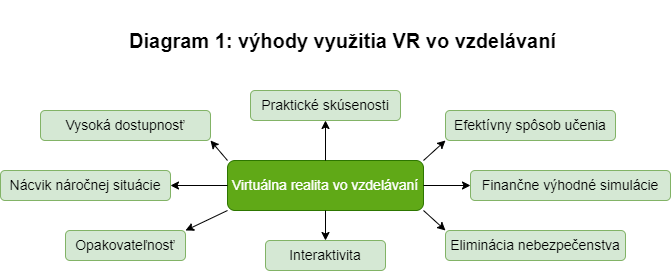
\includegraphics[scale = 0.5]{diagram}

 V ďalších podkapitolách sa budem venovať konkrétnemu využitiu v rámci vyššie spomínaných vekových kategórii a taktiež budem hovoriť o rôznych odvetviach, ktoré dokážu výrazne profitovať zo simulácie reálneho prostredia.

\subsection{Výučba na základnej a strednej škole} \label{deti}
Deti a mladí ľudia nemajú vždy pozitívny prístup k škole a vzdelávaniu a učenie môže byť pre nich náročné, preto by mohlo byť pre školy výhodné zakúpiť niekoľko VR headsetov do jednej miestnosti a počas niektorých hodín poskytnúť zaujímavú formu štúdia naprieč všetkými predmetmi - nemusia si čítať o historickom priebehu bitky počas vojny, môžu si pustiť simuláciu a vidieť historickú udalosť zblízka, nemusia cestovať po svete a sledovať pamiatky, prírodu a metropoly: stačí opäť spustiť vhodnú simuláciu a žiak sa môže ocitnúť na druhej strane zemegule.

\subsection{Výučba vysokoškolských študentov} \label{studenti}
Práve prostredie vysokej školy vidím ako najefektívnejšie využitie možností, ktoré nám poskytuje prostredie virtuálnej reality. Práve v tomto období života sa väčšina ľudí profesijne vyprofiluje a vyberú si odvetvie a prípadne aj konkrétne zamestnanie, ktorému sa chcú v budúcnosti venovať. Prirodzene, v tomto období sa študenti snažia získať všetky možné schopnosti nevyhnutné pre vykonávanie svojej profesie a keďže každá práca je spojená aj s praktickými úkonmi, dokážeme ich pripraviť na väčšinu týchto úkonov už počas štúdia pomocou simulácie vďaka VR. 

Dokonca môžeme tieto simulácie použiť aj na zaujímavejšiu formu teoretického výkladu - bola vykonaná štúdia na pôde univerzity, \cite{studium} ktorá porovnávala bežnú Powerpointovú prezentáciu s VR simuláciou a ukázalo sa, že 70\%  zúčastnených študentov dokázalo vďaka virtuálnej realite preberanú látku lepšie pochopiť  a zapämatať.

Čo sa týka samotných odvetví, využiteľnosť je veľmi široká, preto uvediem tie najzaujímavejšie ako príklad - táto technológia je veľmi obľúbená v medicíne \cite{lekarstvo}, pretože dovoľuje študentom vyskúšať si náročné operácie úplne bezbolestne a bez rizika a taktiež možnosť detailne vidieť rôzne časti tela. Medzi odvetvia so širokým využitím patrí aj inžinierstvo \cite{inzinierstvo}, kde sa dajú simulovať zložité projekty a ich konštrukcia. Výborné využitie zastáva aj v architektúre a návrhu dizajnov \cite{design}, nakoľko je tu možnosť vytvoriť si simuláciu celého návrhu a je vidno, ako návrh vyzerá v celku a vo finálnej podobe.

\subsection{Kurzy pre zamestnancov} \label{zamestnanci}
Výuka sa samozrejme netýka len detí a adolescentov, ale aj dospelých ľudí - môže ísť o nadstavbu štúdia, kurz spojený so zamestnaním alebo rekvalifikáciu. Najväčší úspech by mohla virtuálna realita zožať v rámci kurzov pre zamestnancov, vďaka čomu môže pripraviť ľudí na veľmi špecifickú situáciu a účastník sa naučí, ako počas nej reagovať, pracovať efektívne a vyhnúť sa ohrozeniu. 

Takáto technológie môže pomôcť pri veľkej škále rôznych profesii: týka sa to rôznych kurzov z vyššie spomínaných odvetví v časti vysokoškolskej výučby, taktiež sa týka aj bežných zamestnaní, ale aj takých, kde hrozí vysoké riziko ohrozenia - toto široké spektrum ukazuje uplatnenie technológie VR u polície - existuje hra \cite{policia}, ktorá vznikla v spolupráci s členmi polície a vytvára simuláciu policajných zásahov od riadenia premávky a zastavovania vozidiel až po domáce násilie a ozbrojené lúpeže.

\section{VR a využitie pri špeciálnych požiadavkách výuky} \label{stvrta}

\subsection{Dištančná výuka} \label{pomoc}
Nie je vždy možné, aby bol človek schopný študovať prezenčne, v takom prípade často dochádza k externému štúdiu, prípadne dištančnej forme štúdia kvôli nepriaznivým okolnostiam (napríklad súčasná situácia na Slovensku, kedy je nevyhnutné študovať z domu kvôli pandémii Covidu). Vzhľadom k tomu, že človek nie je osobne prítomný na vyučovaní a nie je možné si viaceré praktické úlohy a experimenty vyskúšať, natíska sa otázka, či by tento problém dokázala vyriešiť virtuálna realita.

Čo sa týka externého štúdia, VR by mohla byť skvelý doplnok k štúdiu. Nakoľko takýto typ štúdia je od začiatku zameraný na dištančnú formu, bolo by možné zadovážiť si potrebnú technológiu na virtuálnu realitu ešte pred začiatkom štúdia a vďaka tomu by bolo vzdelávanie prepojené s priamym kontaktom a schopnosťou vyskúšať mnohé veci, ktoré by sa za normálnych okolností z pohodlia domova nedali vykonávať.

Avšak oproti tomu naša dištančná výuka by teraz nefungovala tak jednoducho - hlavný dôvod je, že nikto nebol na takúto situáciu pripravený a s najväčšou pravdepodobnosťou nemá doma technické vybavenie potrebné na takýto typ výučby. Ďalší problém je v otázke financií, nakoľko je možné, že viacerí študenti by neboli schopní alebo ochotní obetovať danú sumu peňazí za set, ktorý nevyužijú často. 

Napriek tomu si myslím, že so zvyšujúcou sa dostupnosťou a znižujúcou sa cenou VR setu je možné, že v budúcnosti sa z neho stane skoro samozrejmosť v domácnosti, tak ako teraz počítač alebo televízor. V takom prípade by sa aj v takejto náročnej situácii dala udržať veľmi vysoká kvalita štúdia, dokonca by sme sa priblížili čo najautentickejšie k prezenčnej výuke, napríklad dosiahnuť celého univerzitného kampusu \cite{distancne} s možnosťou zúčastňovať sa hodín, písať na tabuľu, diskutovať v skupinách čo by mohol byť skvelý prostriedok pre žiakov aj učiteľov v prípade, že každý musí byť izolovaný doma.

\subsection{Pomoc s učením zdravotne znevýhodnených} \label{pomoc}
Nanešťastie, nie všetci ľudia sa narodia úplne zdraví, prípadne kvôli určitej udalosti počas ich života sa môže stať, že človek je zdravotne znevýhodnený oproti ostatným ľuďom, či už sa jedná o fyzické alebo mentálne znevýhodnenie. Všetci ľudia, ktorý prechádzajú takýmito problémami majú určité prekážky v rámci efektivity bežného spôsobu učenia. Takýmto ľudom dokážeme podať pomocnú ruku a pomôcť im naučiť sa čo najviac vecí, ktoré im môžu pomôcť v živote. 

Ako skvelý príklad by som uviedol situáciu v Číne,\cite{hry} kde sa snažia pomocou hier zaznamenávajúcich pohyb učiť deti, ktoré trpia autizmom a zlepšiť ich kognitívne a sociálne schopnosti. Toto má za výsledok ich lepší vývoj a krok dopredu k väčšej integrácii do spoločnosti.

Je skvelé, že takéto projekty máme možnosť vidieť aj u nás na Slovensku - Technická univerzita v Košiciach a jej tým laboratória LIRKIS pracuje na využití technológie virtuálnej reality pre postihnutých ľudí \cite{svk}, čo umožní lepšie, ľahšie, rýchlejšie pochopenie a zatraktívnenie výučby. Taktiež vedú viaceré semináre, ktoré sa venujú tejto problematike a ukazujú možnosti zlepšenia štúdia pre tých, ktorí s ním majú najviac problémov.

\section{Reakcia na témy z prednášok} \label{piata}
Ešte predtým, ako uzavriem svoje myšlienky ohľadne vzdelávania pomocou virtuálnej reality budem reagovať na viaceré témy, ktoré odzneli počas prednášok na predmete Metódy inžinierskej práce.

\paragraph{Spoločenské súvislosti.}
Žijeme v informačnej dobe a náš život sprevádzajú technológie, ktoré vplývajú na všetko v našom živote a vzdelanie nie je výnimkou - všetko sa zlepšuje a digitalizuje. Virtuálna realita je ďalší krok vo vynovení vzdelávacieho systému a slúži ako základ na výstavbu ďalšieho technologického pokroku vyučovania a ďalších vynálezov, ktoré si teraz možno ani nedokážeme predstaviť.
\paragraph{Historické súvislosti.}
V minulosti sa kvôli ľudským potrebám vytvorili rôzne vynálezy pre skvalitnenie života - požiadavky vo vzdelávaní viedli k tomu, že dnes máme k dispozícii prezentácie na projektoroch, interaktívne tabule, online hodiny, a z potreby dnešnej doby je pravdepodobné, že sa začne bežne využívať virtuálna realita na edukačné účely, čo opäť ukáže, čo ešte potrebujeme zlepšiť na dosiahnutie ideálnej výuky. Naše požiadavky z minulosti formujú budúcnosť a VR bude súčasť tohto cyklu. 
\paragraph{Technológia a ľudia.}
Máme k dispozícii vynikajúcu technológiu vo forme virtuálnej reality, ktorá môže byť prevratná pri vzdelávaní a e teraz je potrebné, aby ľudia konali a veci sa uviedli do pohybu - čím viac ľudí bude ochotných zainvestovať do VR setov, tým rozšírenejším sa stane a ľudia ho spoznajú a pochopia využitie a význam. Taktiež je dôležité, aby ľudia, ktorý určujú chod školstva videli efektivitu tohto vynálezu a spravili maximum, aby ho zaviedli do školských systémov.
 \paragraph{Udržateľnosť a etika.}
Použitie VR na vzdelávacie učenie zahrňuje väčšiu interaktivitu a ponúka iný štýl výuky. Vďaka tomu študenti majú väčší záujem o štúdium, sú pozornejší na hodinách a vzbudzuje v nich túžbu zúčastniť sa týchto hodín, čo vedie k väčšej udržateľnosť študentov. A hoci táto technológia poskytuje určitú zábavu a slobodu na hodine,, v rámci určitých etických pravidiel by študenti nemali zámerne sabotovať simuláciu, prípadne sa správať vulgárne a vytvárať nevhodné výtvory.

\section{Záver} \label{zaver} 
Technológia, ktorú nám prináša virtuálna realita je veľmi prínosná už v tejto dobe naprieč rôznymi vekovými kategóriami a odvetviami a do budúcnosti môžeme predpokladať, že sa objaví ešte viac skvelých využití. Jej vplyv na vyučovanie je už teraz veľký, dokáže vytvoriť omnoho pútavejšie prostredie pre spoznávanie nových faktov, prepojiť teóriu s praxou a tiež poskytnúť simuláciu reálneho problému v určitej profesii. Okrem tohto dokáže pomôcť pri štúdiu, kde sú určité špeciálne podmienky spojené so zdravotným stavom alebo fyzickou neprítomnosťou na vyučovaní. Dá sa povedať, že využitie virtuálnej reality vo vzdelávaní je veľmi dobre rozbehnuté, v posledných rokoch sa tejto téme venuje stále viac ľudí, tejto problematike sa venuje stále viac štúdii a výskumov a bude veľmi zaujímavé sledovať, aké nové edukačné využitia sa budú objavovať v nasledujúcich rokoch. 


%\acknowledgement{Ak niekomu chcete poďakovať\ldots}



\bibliography{literatura}
\bibliographystyle{unsrt}
\end{document}
